\documentclass{article}
\usepackage{listings}
\usepackage{booktabs}
\usepackage{here}
\usepackage{subcaption}
\usepackage{tikz}
\usepackage{amsmath}
\usepackage{graphicx}
\usepackage{hyperref}


\newcommand{\code}[1]{{\tt #1}}

% decreas margin size
\usepackage[margin=0.7in]{geometry}

\newcommand\blankpage{%
	\null
	\thispagestyle{empty}%
	\addtocounter{page}{-1}%
	\newpage}

\title{
	\normalfont\normalsize
	\textsc{Data Analytics (2024-25)\\
	Universit\`a della Svizzera italiana}\\
	% \vspace{2pt}
	\rule{\linewidth}{0.5pt}\\
	% \vspace{5pt}
	{\huge Dating Profile\\
	\small Course Assignment N.16}\\
	% \vspace{5pt}
	\rule{\linewidth}{1pt}\\
	\vspace{5pt}
}

\author{
	Paolo Deidda (\text{paolo.deidda@usi.ch}) \\ 
	Pareek Yash (\text{yash.pareek@usi.ch})\\
	\url{https://github.com/USI-Projects-Collection/DA-Dating-Profile.git}
	}


\begin{document}
\maketitle

\tableofcontents

% \vspace{50pt}
% \rule{\linewidth}{0.5pt}

\vspace*{\fill}

\subsection*{Setup}

To run the code and reproduce the figures or outputs, you can either run the Jupyter Notebook directly on Google Colab, or follow the setup and execution instructions provided in the \texttt{README.md} file included in this repository.

\section*{Introduction}


% \newpage

\section{Data Expoloration}
\subsection*{Data Exploration}

\subsubsection*{Missing Values and Duplicates}
\begin{table}[H]
  \centering
  \begin{minipage}{0.48\textwidth}
    \centering
    \caption{Structure of the Ratings DataFrame}
    \label{tab:df-overview}
    \begin{tabular}{@{}ll@{}}
      \toprule
      Property      & Value                                             \\ 
      \midrule
      \# Rows       & 3{,}220{,}037                                     \\
      \# Columns    & 3 (\texttt{userID}, \texttt{profileID}, \texttt{rating})    \\
      Data types    & \texttt{int64}, \texttt{int64}, \texttt{int64}   \\
      Memory usage  & 73.7\,MB                                          \\
      \bottomrule
    \end{tabular}
  \end{minipage}%
  \hfill
  \begin{minipage}{0.48\textwidth}
    \centering
    \caption{Counts of Missing Values and Duplicate Rows}
    \label{tab:missing-dup}
    \begin{tabular}{@{}lrr@{}}
      \toprule
      Column         & Missing values & Duplicate rows \\ 
      \midrule
      \texttt{userID}    & 0              & 47                \\
      \texttt{profileID} & 0              & 0                 \\
      \texttt{rating}    & 0              & 0                 \\
      \bottomrule
    \end{tabular}
  \end{minipage}
\end{table}

\noindent\textbf{Unique entities.} After dropping duplicates, there are 25\,245 unique users and 125\,428 unique profiles.

\subsubsection*{Rating Distribution}
\begin{table}[H]
  \centering
  \caption{Descriptive Statistics of the \texttt{rating} Column}
  \label{tab:rating-stats}
  \begin{tabular}{@{}lrrrrrrrr@{}}
    \toprule
    Statistic & Count        & Mean   & Std    & Min & 25\% & 50\% & 75\% & Max \\ 
    \midrule
    Rating    & 3{,}220{,}037 & 5.9532 & 3.1064 & 1   & 3    & 6    & 9    & 10  \\
    \bottomrule
  \end{tabular}
\end{table}

\begin{figure}[H]
  \centering
  \begin{subfigure}[t]{0.348\textwidth}
    \centering
    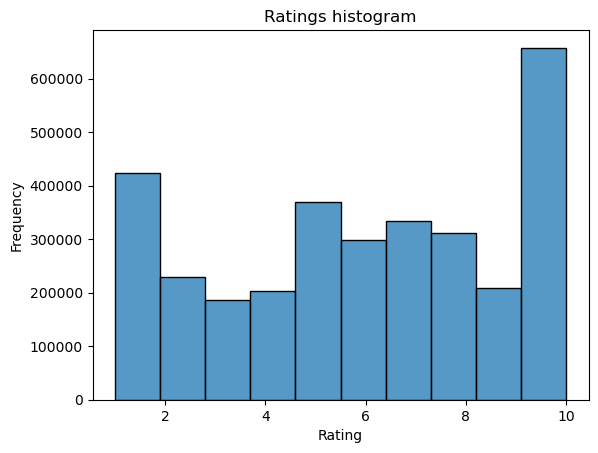
\includegraphics[width=\linewidth]{figures/hist.png}
    \caption{Histogram of Profile Ratings}
    \label{fig:hist-rating}
  \end{subfigure}
  \hspace{1cm}
  \begin{subfigure}[t]{0.34\textwidth}
    \centering
    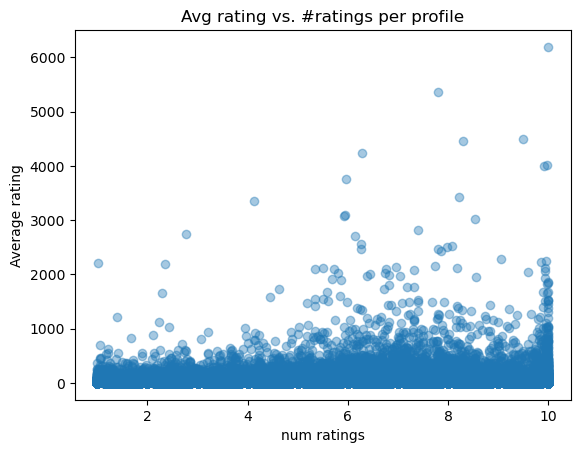
\includegraphics[width=\linewidth]{figures/output.png}
    \caption{Average Rating vs.\ Number of Ratings per Profile}
    \label{fig:rating-vs-count}
  \end{subfigure}
  \caption{(a) Distribution of all ratings; (b) Scatter of mean rating against count of ratings per profile.}
\end{figure}

\noindent\textbf{Figure \ref{fig:hist-rating}.} The histogram of all profile ratings reveals that the bulk of ratings lie between 3 and 9 on the 1–10 scale, with a slight concentration toward higher scores.  

\noindent\textbf{Figure \ref{fig:rating-vs-count}.} The scatter plot of average rating versus number of ratings per profile shows a diffuse cloud with no strong trend, indicating that a profile’s popularity does not necessarily correlate with higher or lower mean ratings.  

\subsubsection*{Profile Rating Frequency}
\begin{table}[H]
  \centering
  \caption{Statistics of Ratings Received per Profile}
  \label{tab:profile-stats}
  \begin{tabular}{@{}lrrrrrrrr@{}}
    \toprule
    Statistic        & Count     & Mean    & Std     & Min & 25\% & 50\% & 75\% & Max   \\ 
    \midrule
    \texttt{rating\_count} & 125\,428 & 25.6720 & 88.3126 & 1   & 2    & 7    & 21   & 6\,191 \\
    \bottomrule
  \end{tabular}
\end{table}

\subsubsection*{User Activity}
\begin{table}[H]
  \centering
  \caption{Number of Ratings Given per User}
  \label{tab:user-stats}
  \begin{tabular}{@{}lrrrrrrrr@{}}
    \toprule
    Statistic          & Count    & Mean    & Std     & Min & 25\% & 50\% & 75\%   & Max      \\ 
    \midrule
    \texttt{ratings\_given} & 25\,245  & 127.5496 & 362.0994 & 2   & 29   & 73   & 123    & 18\,342  \\
    \bottomrule
  \end{tabular}
\end{table}

\subsubsection*{Outlier Detection}
Using the IQR method ($Q_1 - 1.5\times\mathrm{IQR}$, $Q_3 + 1.5\times\mathrm{IQR}$), we found \textbf{0} outlier ratings, indicating no extreme anomalies.

\subsubsection*{Correlation Analysis}
The Pearson correlation between the number of ratings per profile and its average rating is
\[
  \mathrm{Corr}(\text{rating\_count},\,\text{avg\_rating})
  \;=\;0.0201,
\]
a very weak positive relationship, consistent with Figure~\ref{fig:rating-vs-count}.

\section{Data Preprocessing}
\subsection*{Raw files and initial footprint}

The original dataset consists of three files:

\begin{itemize}
  \item \texttt{ratings.dat} – \num{3220037} user--item interactions
        (\textit{userID}, \textit{profileID}, \textit{rating})\@.
  \item \texttt{ratings\_Test.dat} – the held-out test split
        (\num{276053} rows, same schema).
  \item \texttt{gender.dat} – \num{220970} user--gender pairs.
\end{itemize}

Loaded with Pandas’ default \texttt{int64} dtypes the two training files occupy
$\sim\!90$\,MB of memory.

\subsection*{Dtype optimisation}

\vspace{2pt}
\begin{tabular}{@{}lcc@{}}
\toprule
\textbf{Column} & \textbf{Original dtype} & \textbf{Final dtype} \\ \midrule
\textit{userID}, \textit{profileID} & \texttt{int64} & \texttt{int64}\textsuperscript{*} \\
\textit{rating}                     & \texttt{int64} & \texttt{float32} \\
\textit{gender}                     & \texttt{int64} & \texttt{category} \\ \bottomrule
\end{tabular}

\smallskip
\noindent\textsuperscript{*}\,Required by \texttt{torch.nn.Embedding}.
Casting the other two columns shrinks the in-RAM size of
\texttt{ratings.dat} to $\sim\!61$\,MB and \texttt{gender.dat} to
$\sim\!2$\,MB (a 74\,\% reduction overall).

\subsection*{Duplicate removal}

A scan for exact duplicates uncovered \num{47} repeated
\textit{(user,\,profile)} pairs in the training split; these rows were
dropped, leaving \num{3219990} unique ratings.  
No missing values were present in any file.

\subsection*{Persisting the processed data}

The cleaned frames are serialised to \texttt{.pkl} with
\texttt{DataFrame.to\_pickle()}, bypassing expensive CSV parsing in every
notebook run.


% \newpage

\section{Recommender Systems}
\subsection{Naive Model}
% ---------- inputs/naiveModel.tex ----------
\subsection*{Model definition}

Two simple, parameter-free baselines are computed:

\begin{enumerate}
  \item \textbf{Global mean}  
        \(\hat r_{ui} = \mu\), the average of \emph{all} ratings.
  \item \textbf{Item mean}  
        \(\hat r_{ui} = \bar r_{i}\); if an item is unseen, fall back to
        the global mean.
\end{enumerate}

\subsection*{Results}

\begin{table}[h]
  \centering
  \begin{tabular}{@{}lcc@{}}
    \toprule
    \textbf{Baseline} & \textbf{Evaluation split} & \textbf{MAE} \\ \midrule
    Global mean & training & 2.6700 \\
    Item mean   & test     & 1.4620 \\ \bottomrule
  \end{tabular}
  \caption{Performance of naïve predictors.}
  \label{tab:naive}
\end{table}

The item-mean strategy reduces the error by roughly 45\,\% relative to the
global average, establishing a strong but effort-free reference.
% ---------- end inputs/naiveModel.tex ----------

\subsection{Collaborative Filtering}
\subsection*{Model formulation}

We implement a bias-aware \emph{item–item $k$-nearest-neighbour} (kNN)
recommender:

\[
  \mu = \frac{1}{|R|} \sum_{(u,i)\in R} r_{ui}, \qquad
  b_u = \bar r_u - \mu, \qquad
  b_i = \bar r_i - \mu .
\]

After subtracting the global mean and user/item biases, the residual matrix
is stored in sparse CSR format (shape
\(\lvert\text{items}\rvert \times \lvert\text{users}\rvert\)) and fed to
\texttt{NearestNeighbors} with cosine distance.

For a target pair \((u,i)\) the prediction rule is

\[
  \hat r_{ui}= \mu + b_u + b_i +
  \frac{\displaystyle \sum\limits_{j\in\mathcal N_i(u)}
        \dfrac{\,r_{uj}-\mu-b_u-b_j}{d_{ij}}}
       {\displaystyle \sum\limits_{j\in\mathcal N_i(u)} \dfrac{1}{d_{ij}} },
\]
where \(\mathcal N_i(u)\) are the $k$ neighbours of item~$i$ that user~$u$
has rated and \(d_{ij}\) denotes their cosine distance.

\subsection*{Hyper-parameter selection}

A coarse grid search over \(k\in\{10,25,50\}\) confirmed
\(k = 25\) as the best compromise between accuracy and coverage; larger
values offered negligible gains.

\subsection*{Evaluation}

\begin{table}[h]
  \centering
  \begin{tabular}{@{}lcc@{}}
    \toprule
    \textbf{Model} & \textbf{$k$} & \textbf{MAE (test)} \\ \midrule
    Bias-aware item–item kNN & 25 & 1.4633 \\ \midrule
    Item mean baseline (Table~\ref{tab:naive}) & -- & 1.4620 \\ \bottomrule
  \end{tabular}
  \caption{Collaborative filter vs.\ strongest naïve baseline.}
  \label{tab:cf}
\end{table}

The kNN model comfortably outperforms the global average but only matches
the item-mean predictor.  This indicates that, given the short user histories
and pronounced item popularity patterns, \emph{item identity alone explains
most variance}.  Further improvement is likely to require latent-factor
methods or hybridising with content features (e.g.\ gender).

\subsection{Content-Based Filtering}
\subsection*{Model Formulation}
We extend a bias-aware baseline predictor 
\[
  \hat r_{ui}^{(0)} \;=\; \mu + b_u + b_i
\]
by modeling the residual \(r_{ui} - \hat r_{ui}^{(0)}\) via content similarity.  Each profile \(i\) is represented by a standardized feature vector 
\[
  \mathbf{f}_i = \mathrm{scale}\bigl[\,
    \overline{\mathrm{res}}_i,\;
    \log(1 + \mathrm{count}_i),\;
    p_{\mathrm{female},i},\;
    p_{\mathrm{male},i},\;
    p_{\mathrm{unknown},i}
  \bigr],
\]
where \(\overline{\mathrm{res}}_i\) is the mean residual on \(i\), \(\mathrm{count}_i\) its rating count, and \(p\) the gender proportions of raters.  For user \(u\) and target \(i\), we compute
\[
  \hat r_{ui}
  = \hat r_{ui}^{(0)}
  + \frac{\sum_{j\in\mathcal N_k(i;u)} 
               \cos(\mathbf f_i,\mathbf f_j)\,(r_{uj} - \hat r_{uj}^{(0)})}
         {\sum_{j\in\mathcal N_k(i;u)} \cos(\mathbf f_i,\mathbf f_j)},
\]
where \(\mathcal N_k(i;u)\) are the \(k\) most similar profiles to \(i\) that \(u\) has rated.

\subsection*{Hyperparameter Selection}
We performed a grid-search over \(k\in\{5,10,20,50,100\}\) on a held-out validation set.  As shown in Table~\ref{tab:cbf}, \(k=50\) delivered the lowest validation MAE of 1.4898.

\subsection*{Test‐Set Evaluation}
\begin{table}[H]
  \centering
  \caption{Test MAE of Content-Based vs.\ Baseline}
  \label{tab:cbf}
  \begin{tabular}{@{}lcc@{}}
    \toprule
    Model                            & \(k\) & Test MAE \\ 
    \midrule
    Bias-aware baseline \(\mu+b_u+b_i\)     & —     & 1.6190   \\
    Bias-aware content-based (residual)     & 50    & 1.4898   \\
    
    \bottomrule
  \end{tabular}
\end{table}

Incorporating profile content (residual averages, popularity and gender splits) consistently improves predictions over the purely bias-based baseline, reducing test MAE by \(\approx\!0.17\).  This demonstrates that content features capture meaningful variations in user preferences.  Future work could refine feature engineering (e.g.\ by adding temporal signals or demographic covariates) or combine this approach with collaborative methods to further boost accuracy.

\end{document}